\RequirePackage{amsmath,mathtools}
\documentclass[a4paper,10pt,department=FakEI]{OTHRartcl}

% ==============================================================================
% PAKETE & EINSTELLUNGEN
% ==============================================================================
\usepackage{iftex}
\ifTUTeX
\else
    \usepackage[utf8]{inputenc}
    \usepackage[T1]{fontenc}
    \usepackage{amssymb}
\fi
\usepackage[ngerman]{babel}
\usepackage{geometry}
\usepackage{graphicx}
\usepackage{booktabs}
\usepackage{tabularx}
\usepackage{array}
\usepackage{xcolor}
\usepackage{float}
\usepackage{tcolorbox}
\tcbuselibrary{skins,breakable}
\usepackage{caption}
\usepackage{tikz}
\usetikzlibrary{shapes,arrows.meta,positioning,calc}
\usepackage{hyperref}
\usepackage[
    headsepline=0.4pt,
    footsepline=0.4pt,
    plainfootsepline=true
]{scrlayer-scrpage}

% Seitengeometrie
\geometry{
    a4paper,
    top=18mm,
    bottom=18mm,
    left=18mm,
    right=18mm,
    headheight=14pt,
    headsep=5mm,
    footskip=8mm
}
\setlength{\footheight}{20pt}

% OTH-Farben
\definecolor{primaryBlue}{RGB}{0, 75, 135}
\definecolor{darkgray}{RGB}{50, 50, 50}
\definecolor{lightgray}{RGB}{246, 248, 251}
\definecolor{accentOrange}{RGB}{235, 115, 35}

% Hyperref Setup
\hypersetup{
    colorlinks=true,
    linkcolor=primaryBlue,
    citecolor=primaryBlue,
    urlcolor=primaryBlue,
    pdftitle={Versuch V2: Modellbildung Drosselklappe - Regelungstechnik Anwendungen},
    pdfauthor={Johannes Wutz, Oliver Grundmann, Eduardo Llama}
}

% Bildunterschriften
\captionsetup{
    font={small},
    labelfont={bf,color=primaryBlue},
    labelsep=colon,
    skip=3pt
}

% Tabellenabstände
\renewcommand{\arraystretch}{1.12}

% Boxen-Design
\tcbset{
    enhanced,
    colback=lightgray,
    colframe=primaryBlue!35,
    boxrule=0.6pt,
    arc=1.5mm,
    left=3mm, right=3mm, top=2mm, bottom=2mm
}

% Kopf- und Fußzeilen (Scrlayer-Scrpage)
\clearpairofpagestyles
\ihead{\textsf{\small Regelungstechnik Anwendungen $\cdot$ Versuch V2: Modellbildung Drosselklappe}}
\ohead{\textsf{\small Gruppe 2}}
\cfoot[\raisebox{-2.5mm}{\textsf{\thepage\ von \pageref*{doc:lastpage}}}]{\raisebox{-2.5mm}{\textsf{\thepage\ von \pageref*{doc:lastpage}}}}
\pagestyle{scrheadings}

% Absatzformatierung
\setlength{\parindent}{0pt}
\setlength{\parskip}{2.5pt}

% Inhaltsverzeichnis Konfiguration
\setcounter{tocdepth}{2}
\setcounter{secnumdepth}{2}
\addto\captionsngerman{\renewcommand*{\contentsname}{Inhalt}}
\deftocheading{toc}{\noindent{\Large\bfseries #1}\par\vspace{2.5mm}}

\DeclareTOCStyleEntry[
    linefill=\TOCLineLeaderFill,
    beforeskip=2.5pt plus 1pt,
    entrynumberformat=\bfseries,
    entryformat=\bfseries,
    pagenumberformat=\bfseries
]{tocline}{section}

\DeclareTOCStyleEntry[
    linefill=\TOCLineLeaderFill,
    beforeskip=0.5pt,
    indent=1.5em,
    numwidth=2.2em
]{tocline}{subsection}

% ==============================================================================
% DOKUMENTENBEGINN
% ==============================================================================
\begin{document}

% ##############################################################################
% SEITE 1: DECKBLATT NACH VORLAGE DER VERSUCHSANLEITUNG
% ##############################################################################
\thispagestyle{plain}

\noindent
\begin{minipage}[c]{0.55\textwidth}
    \TheLogo
\end{minipage}%
\begin{minipage}[c]{0.45\textwidth}
    \raggedleft
    {\fontsize{13}{16}\selectfont\bfseries Regelungstechnik Anwendungen}\\[1.5mm]
    {\normalsize Prof. Dr. Brüdigam}
\end{minipage}

\vspace{7mm}

\begin{center}
    {\fontsize{18}{22}\selectfont\bfseries Versuch V2: Modellbildung Drosselklappe}
\end{center}

\vspace{4mm}

\begin{tcolorbox}[
    sharp corners,
    colback=white,
    colframe=black,
    boxrule=0.7pt,
    left=8mm, right=8mm, top=5.5mm, bottom=5.5mm
]
\fontsize{10.5}{16}\selectfont
\noindent
Studiengang:\,\underline{\makebox[5.6cm][l]{\strut\hspace{1.5mm}\textbf{Elektro- und Informationstechnik}}}
\hspace{9mm}
Versuchsdatum:\,\underline{\makebox[3.0cm][l]{\strut\hspace{1.5mm}\textbf{09.11.2026}}}

\vspace{4.5mm}
\noindent
Gruppen-Nr.:\,\underline{\makebox[5.6cm][l]{\strut\hspace{1.5mm}\textbf{2}}}

\vspace{4.5mm}
\noindent
Teilnehmer:\,\underline{\makebox[5.6cm][l]{\strut\hspace{1.5mm}\textbf{Johannes Wutz}}}

\vspace{2.8mm}
\noindent
\hphantom{Teilnehmer:\,}\underline{\makebox[5.6cm][l]{\strut\hspace{1.5mm}\textbf{Oliver Grundmann}}}

\vspace{2.8mm}
\noindent
\hphantom{Teilnehmer:\,}\underline{\makebox[5.6cm][l]{\strut\hspace{1.5mm}\textbf{Eduardo Llama}}}
\end{tcolorbox}

\vspace{5mm}

\begingroup
\hypersetup{linkcolor=black}
\tableofcontents
\endgroup

\clearpage

% ##############################################################################
% SEITE 2: GRUNDLAGEN & SYSTEMBESCHREIBUNG
% ##############################################################################
\section{Grundlagen und Systembeschreibung}
\subsection{Ziel des Versuchs}
Ziel des Versuchs ist die physikalisch-mathematische Modellbildung einer elektrisch betätigten Drosselklappe (Elektronisches Gaspedal, E-Gas) eines Ottomotors sowie deren Umsetzung und Verifikation in MATLAB/Simulink. Hierzu werden die elektrischen und mechanischen Systemparameter experimentell am realen Bauteil sowie anhand von Oszilloskop-Messungen ermittelt, auf Plausibilität geprüft und durch Gegenüberstellung des simulierten und realen Öffnungsvorgangs bei $U = 6\,\text{V}$ validiert.

\subsection{Systemaufbau und Nichtlinearitäten der elektrischen Drosselklappe}
Die Drosselklappe reguliert den in den Verbrennungsmotor einströmenden Luftmassenstrom im Stellbereich von $\varphi_{\text{DK}} = 0^\circ \dots 90^\circ$. Ein permanenterregter Gleichstrommotor treibt die Klappenwelle über ein Untersetzungsgetriebe ($k_{\text{Gr}} = 1/i$) an, während ein Istwert-Potentiometer den aktuellen Öffnungswinkel erfasst. Das Systemverhalten wird maßgeblich durch zwei starke Nichtlinearitäten geprägt:
\begin{itemize}
    \item \textbf{Vorgespannte Notlauffeder (Fail-Safe):}\\
    Bei unbestromtem Motor zieht ein doppelt wirkendes Federsystem die Klappe in eine definierte Notlaufposition ($\varphi_{\text{NLP}} = 7{,}5^\circ$), um im Fehlerfall einen sicheren Notbetrieb des Motors zu gewährleisten. Da die Feder gegen einen festen Anschlag vorgespannt ist, bewirkt sie beim Verlassen der Notlaufposition einen abrupten Momentensprung (Unstetigkeit bei $\varphi_{\text{NLP}}$).
    \item \textbf{Festkörperreibung und mechanische Anschläge:}\\
    In den Wellenlagern, den Kohlebürsten des Kommutators sowie den Zahnrädern tritt ausgeprägte Haft- und Gleitreibung ($M_R$) auf, die jeder Bewegung entgegenwirkt. Zudem begrenzen steife mechanische Anschläge bei $0^\circ$ und $90^\circ$ den Drehwinkel; ein ungedämpftes Anschlagen bei Spannungen $> 6\,\text{V}$ kann zum Abreißen der Kunststoff-Getriebezähne führen.
\end{itemize}

\subsection{Mathematische Modellbildung und Simulink-Struktur}
Aus der Maschengleichung des Ankerkreises $u(t) = R \cdot I(t) + L \cdot \frac{\mathrm{d}I(t)}{\mathrm{d}t} + u_{\text{EMK}}(t)$ folgt im Bildbereich mit der elektrischen Zeitkonstante $\tau_{\text{el}} = L/R$ das $\text{PT}_1$-Übertragungsverhalten für den Motorstrom $I(s)$:
\begin{equation}
    I(s) = \frac{1/R}{\frac{L}{R}\,s + 1} \cdot \bigl(U(s) - U_{\text{EMK}}(s)\bigr) \quad \text{mit} \quad u_{\text{EMK}}(t) = k_{\text{EMK}} \cdot \omega(t)
\end{equation}
Das elektromagnetische Antriebsmoment $M_A = k_{\text{Mot}} \cdot I$ (mit $k_{\text{Mot}} = c \cdot \Phi_E$) wird an der Motorwelle um das geschwindigkeitsabhängige Reibmoment $M_R(\omega) = M_{R0} \cdot \operatorname{sgn}(\omega)$ und das winkelabhängige Federmoment $M_F(\varphi_{\text{DK}})$ reduziert. Über den Drallsatz der Rotation ergibt sich die Winkelbeschleunigung $\dot{\omega}$ des Motors und nach zweifacher Integration sowie Multiplikation mit dem Getriebefaktor $k_{\text{Gr}}$ der Klappenwinkel $\varphi_{\text{DK}}$:
\begin{equation}
    \dot{\omega}(t) = \frac{1}{J} \cdot \bigl(M_A(t) - M_R(\omega) - M_F(\varphi_{\text{DK}})\bigr) \implies \varphi_{\text{DK,deg}}(s) = \frac{180^\circ}{\pi} \cdot k_{\text{Gr}} \cdot \frac{1}{s^2} \cdot \dot{\Omega}(s)
\end{equation}

\begin{figure}[H]
\centering
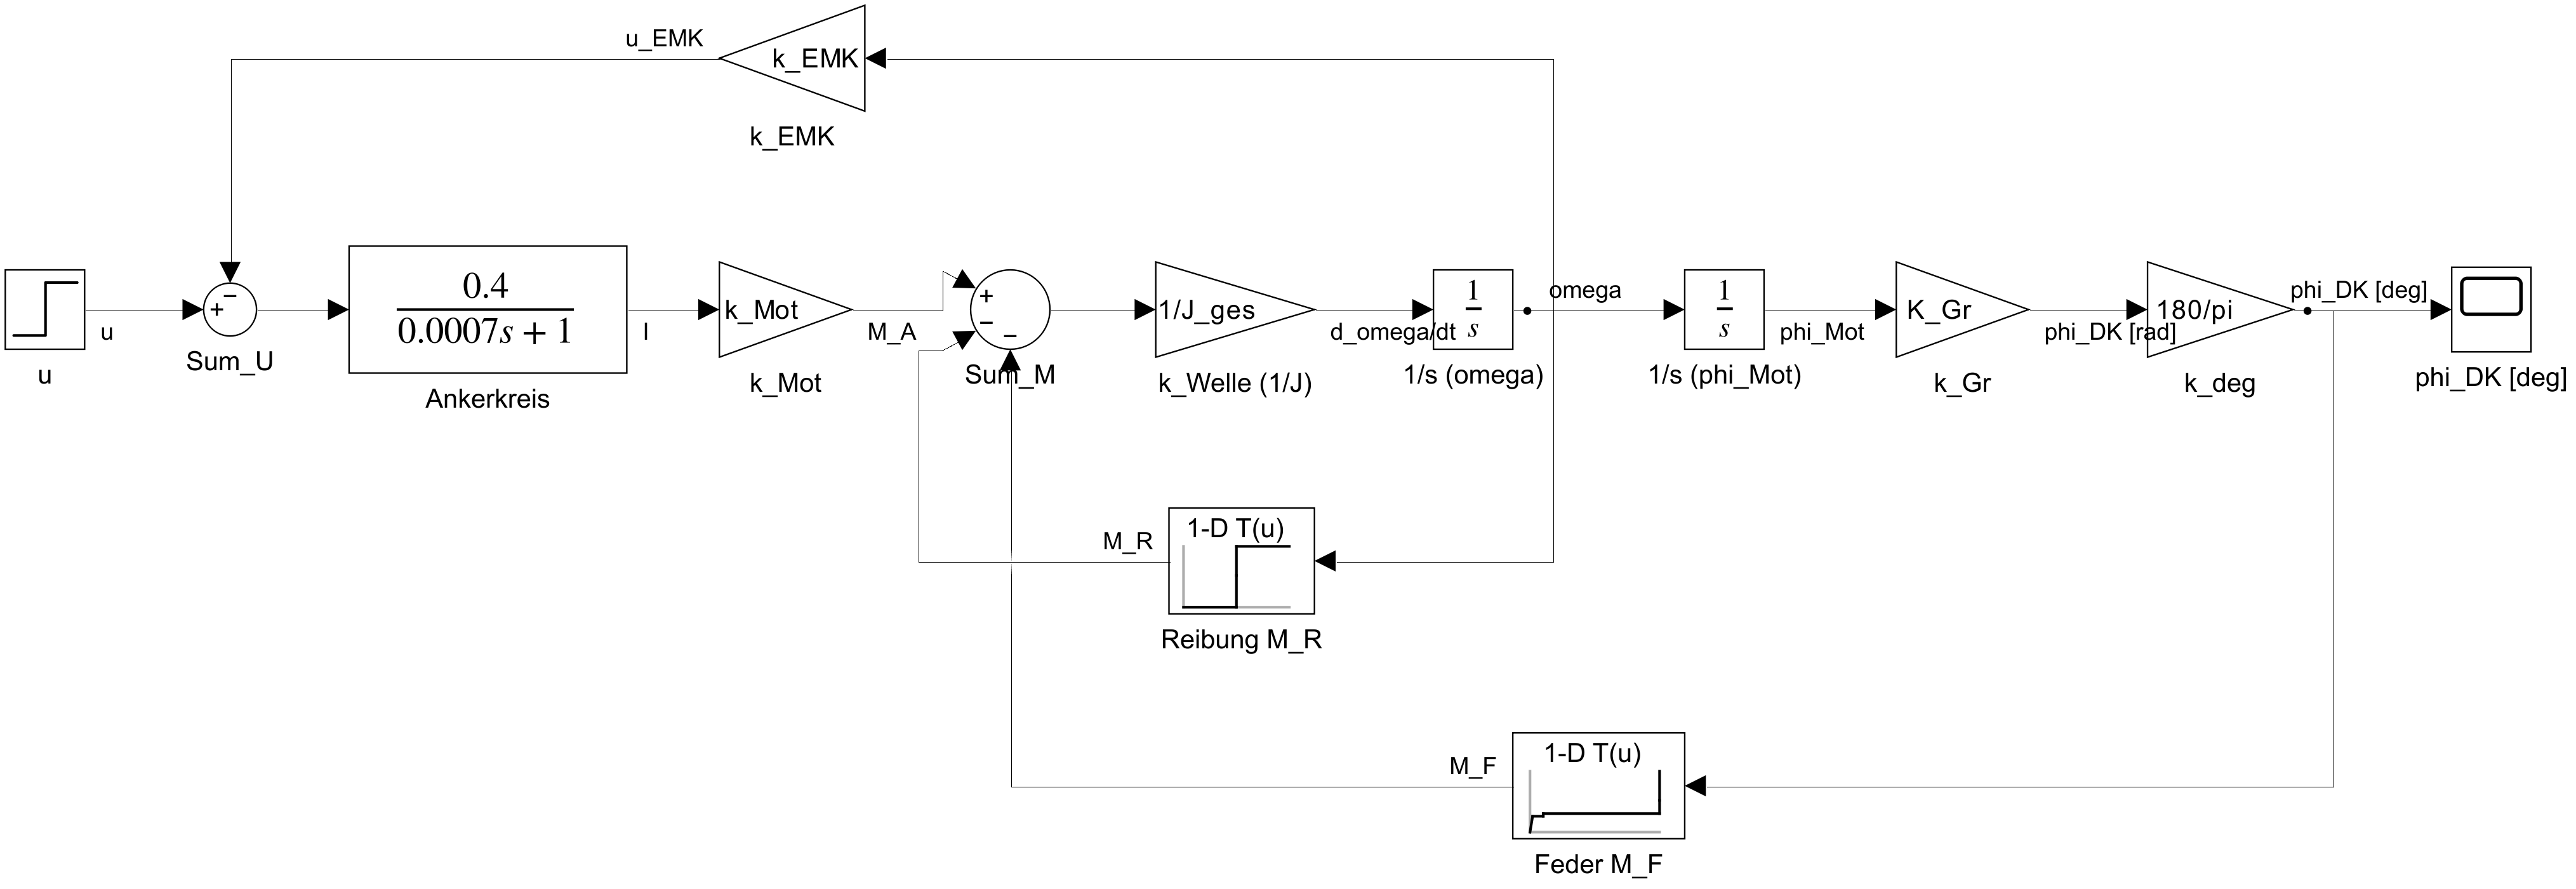
\includegraphics[width=\textwidth,height=5.8cm,keepaspectratio]{simulink_modell_drosselklappe.png}
\caption{In MATLAB/Simulink aufgebautes Gesamtmodell der elektrischen Drosselklappe}
\label{fig:simulink_drosselklappe}
\end{figure}

\clearpage

% ##############################################################################
% SEITE 3: EXPERIMENTELLE PARAMETERBESTIMMUNG
% ##############################################################################
\section{Experimentelle Parameterbestimmung}
\subsection{Messverfahren zur Bestimmung der Modellparameter}
Die Parameter der einzelnen Systemblöcke wurden durch Kombination elektrischer, mechanischer und geometrischer Messverfahren bestimmt:
\begin{itemize}\setlength{\itemsep}{2pt}
    \item \textbf{Ankerwiderstand $R$:}\\
    Eine direkte Widerstandsmessung mit dem Multimeter ist durch Übergangswiderstände (Kohlebürsten, Oxidschicht und Verschmutzung am Kommutator) fehlerbehaftet. Daher wird der Rotor im Stillstand festgehalten ($\omega = 0 \implies u_{\text{EMK}} = 0\,\text{V}$) und an den Anschlüssen in verschiedenen Winkelstellungen (verschiedene Kommutatorlamellen) ein definierter Betriebsstrom von $I = 1\,\text{A}$ eingeprägt. Aus $R = U/I$ folgt direkt $|R| = |U| = 2{,}5\,\Omega$ (wobei der Widerstand bei längerer Bestromung durch Erwärmung leicht ansteigt).

    \item \textbf{Ankerinduktivität $L$:}\\
    Die Messung kann zunächst mit einem RLC-Messgerät über den Wechselstromwiderstand bei einer Prüffrequenz von $f = 1\,\text{kHz}$ erfolgen. Näher am realen Normalbetrieb ist jedoch die Messung über einen Spannungssprung auf $U = 6\,\text{V}$ und Aufzeichnung des Stromverlaufs $I(t)$ am Oszilloskop bei festgehaltenem Rotor ($\omega = 0$, Abbildung~\ref{fig:oszi_messungen} links), da hierbei mit dem realen Betriebsstrom ohne Einfluss von Verschmutzung oder Oxidschichten und ohne hohe Prüffrequenz gemessen wird. Mit der aus dem Oszilloskop bestimmten elektrischen Zeitkonstante $\tau_{\text{el}} = 0{,}625\,\text{ms}$ berechnet sich die Induktivität zu:
    \begin{equation}
        L = R \cdot \tau_{\text{el}} = 2{,}5\,\Omega \cdot 0{,}625\,\text{ms} = 1{,}56\,\text{mH}
    \end{equation}

    \item \textbf{Getriebefaktor $k_{\text{Gr}}$:}\\
    Zur Bestimmung des Getriebefaktors werden die Zähne aller beteiligten Zahnräder des Getriebes gezählt und daraus das Gesamtübersetzungsverhältnis gebildet. Mit einer Untersetzung von $i = 20$ ergibt sich:
    \begin{equation}
        k_{\text{Gr}} = \frac{\varphi_{\text{DK}}}{\varphi_{\text{Mot}}} = \frac{1}{i} = \frac{1}{20} = 0{,}05
    \end{equation}

    \item \textbf{Reibmoment $M_R$ und Federkennlinie $M_F$:}\\
    Mit einem Kraftmesser wird die benötigte Kraft beim langsamen Öffnen und beim langsamen Schließen der Klappe gemessen. Da die Reibkraft $F_R$ stets der jeweiligen Bewegungsrichtung entgegenwirkt, während die Federkraft $F_F$ immer in Richtung der Notlaufposition zieht, gilt für die gemessene Gesamtkraft beim Öffnen ($F_{\text{ges,auf}}$) und beim Schließen ($F_{\text{ges,zu}}$):
    \begin{equation}
        F_{\text{ges,auf}} = F_F + F_R, \qquad F_{\text{ges,zu}} = F_F - F_R
    \end{equation}
    Durch Addition bzw. Subtraktion der beiden Gleichungen lassen sich Feder- und Reibkraft mathematisch separieren und mit dem Hebelarm $r$ sowie dem Getriebefaktor $k_{\text{Gr}}$ auf die Motorwelle umrechnen:
    \begin{align}
        F_{\text{ges,auf}} + F_{\text{ges,zu}} = 2\,F_F &\implies F_F = \frac{F_{\text{ges,auf}} + F_{\text{ges,zu}}}{2} \\
        F_{\text{ges,auf}} - F_{\text{ges,zu}} = 2\,F_R &\implies F_R = \frac{F_{\text{ges,auf}} - F_{\text{ges,zu}}}{2}
    \end{align}
    Bezogen auf die Motorwelle ($M_{\text{Mot}} = F \cdot r \cdot k_{\text{Gr}}$) ergibt sich daraus ein konstantes Reibmoment von $M_R = 0{,}008\,\text{Nm}$. Für das Federmoment werden zwei Winkelpositionen ausgewertet: An der Notlaufposition ($\varphi_{\text{NLP}} = 7{,}5^\circ$) springt das Federmoment durch die Vorspannung auf $M_{F,\text{NLP}} = 0{,}015\,\text{Nm}$ und steigt bis zum Anschlag ($\varphi_{90^\circ} = 90^\circ$) auf $M_{F,90^\circ} = 0{,}022\,\text{Nm}$ an. Die Federkonstante $c_F$ ergibt sich als Steigung der Kennlinie zwischen diesen beiden Positionen:
    \begin{equation}
        c_F = \frac{M_{F,90^\circ} - M_{F,\text{NLP}}}{90^\circ - \varphi_{\text{NLP}}} = \frac{0{,}022\,\text{Nm} - 0{,}015\,\text{Nm}}{90^\circ - 7{,}5^\circ} = \frac{0{,}007\,\text{Nm}}{82{,}5^\circ} = 8{,}48 \cdot 10^{-5}\,\frac{\text{Nm}}{^\circ}
    \end{equation}

    \item \textbf{Motormomentkonstante $k_{\text{Mot}}$:}\\
    Zunächst wird das mechanische Moment bestimmt, um die Klappe zu öffnen, und anschließend der Motorstrom $I$ gemessen, der für die gleiche Bewegung benötigt wird. Alternativ lässt sich die Konstante über Differenzgrößen bestimmen, also über eine Kraftänderung $\Delta F$ und die zugehörige Stromänderung $\Delta I$. Da das mechanische Moment an der Drosselklappe gemessen wird, jedoch das elektrische Moment des Motors gefragt ist und das Getriebe dazwischen liegt, muss der Getriebefaktor $k_{\text{Gr}}$ berücksichtigt werden:
    \begin{equation}
        k_{\text{Mot}} = \frac{\Delta M_{\text{Mot}}}{\Delta I} = \frac{\Delta M_{\text{Klappe}} \cdot k_{\text{Gr}}}{\Delta I} = \frac{\Delta F \cdot r \cdot k_{\text{Gr}}}{\Delta I} = 0{,}027\,\frac{\text{Nm}}{\text{A}}
    \end{equation}

    \item \textbf{Massenträgheitsmoment $J$:}\\
    Eine Bestimmung über Ein- und Ausgangsgröße ist nicht sinnvoll, da die Winkelbeschleunigung $\dot{\omega}$ messtechnisch nicht gut darstellbar ist. Stattdessen wird das Trägheitsmoment über die Geometrie und das Gewicht der einzelnen Komponenten berechnet und zusammengefügt ($J = \frac{1}{2} m r^2$). Da sich die Klappe im Vergleich zum Rotor um den Getriebefaktor $k_{\text{Gr}}$ langsamer bewegt und der Faktor $k_{\text{Gr}}$ sowohl über das Moment als auch über die Drehzahl eingeht, werden die Trägheitsmomente der langsamen Teile mit $k_{\text{Gr}}^2$ auf die Motorwelle umgerechnet. Da diese Anteile durch die langsame Bewegung verschwindend klein sind und der Rotor als Vollzylinder ohnehin etwas zu groß bestimmt wird, ist nur das Trägheitsmoment des Rotors relevant:
    \begin{equation}
        J_{\text{ges}} = J_{\text{Rotor}} + k_{\text{Gr}}^2 \cdot J_{\text{Klappe}} \approx J_{\text{Rotor}} = 7{,}2 \cdot 10^{-6}\,\text{kg\,m}^2
    \end{equation}
\end{itemize}

% ##############################################################################
% SEITE 4: EMK-BESTIMMUNG, PARAMETERÜBERSICHT & PLAUSIBILISIERUNG
% ##############################################################################
\subsection{Bestimmung der EMK-Konstante \texorpdfstring{$k_{\text{EMK}}$}{k\_EMK} auf zwei Wegen}
Eine bekannte konstante Drehzahl aufzugeben und an den Klemmen die Spannung zu messen ist nicht möglich, da die Klappe sonst sofort an den mechanischen Anschlag fährt. Daher wird die Klappe im stromlosen Zustand von der Notlaufposition ($\varphi_{\text{NLP}} = 7{,}5^\circ$) bis zum Anschlag ($90^\circ$, also $\Delta\varphi_{\text{DK}} = 82{,}5^\circ = 1{,}440\,\text{rad}$) von Hand aufgedrückt und die induzierte Klemmenspannung am Oszilloskop aufgezeichnet (Abbildung~\ref{fig:oszi_messungen} Mitte und Rechts):

\begin{figure}[H]
\centering
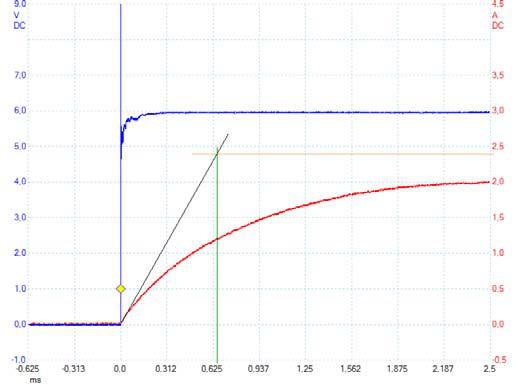
\includegraphics[width=0.33\textwidth,height=3.4cm,keepaspectratio]{oszi_p1_1.png}\hfill
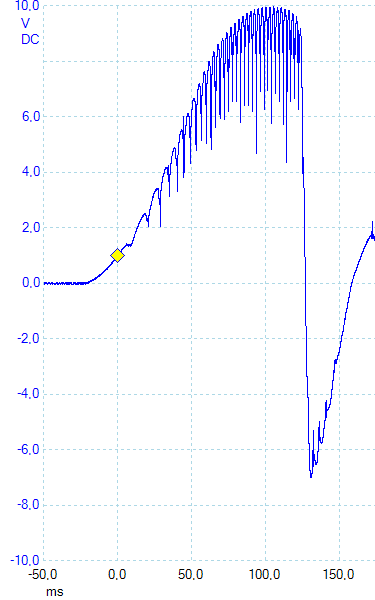
\includegraphics[width=0.31\textwidth,height=3.4cm,keepaspectratio]{oszi_p1_2.png}\hfill
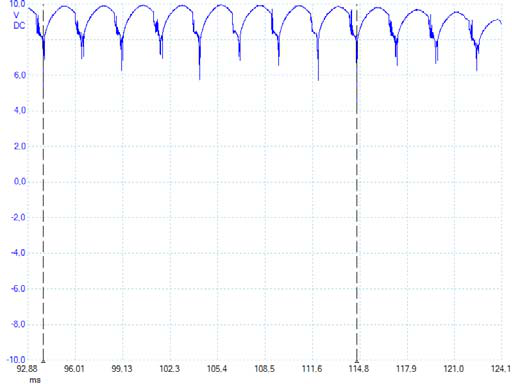
\includegraphics[width=0.33\textwidth,height=3.4cm,keepaspectratio]{oszi_p1_3.png}
\caption{Oszilloskop-Messungen: Ankerzeitkonstante $\tau_{\text{el}}$ bei $6\,\text{V}$ (links), induzierte EMK beim manuellen Aufdrücken von $7{,}5^\circ \to 90^\circ$ (Mitte) sowie Ausschnittvergrößerung der Kommutator-Oberschwingungen bei 8 Rotorlamellen (rechts).}
\label{fig:oszi_messungen}
\end{figure}
\begin{enumerate}\setlength{\itemsep}{2pt}
    \item \textbf{Methode 1 (Über mittlere Winkelgeschwindigkeit und mittlere Spannung):}\\
    Aus der Oszilloskop-Aufnahme des Öffnungsvorgangs von $7{,}5^\circ$ bis $90^\circ$ (Abbildung~\ref{fig:oszi_messungen} Mitte) wird die Dauer der Bewegung $\Delta t \approx 125\,\text{ms} = 0{,}125\,\text{s}$ sowie die mittlere Spannung $\bar{u}_{\text{EMK}} \approx 6{,}9\,\text{V}$ abgelesen. Über den Getriebefaktor $k_{\text{Gr}} = 0{,}05$ ergibt sich der zurückgelegte Drehwinkel des Motors zu $\Delta\varphi_{\text{Mot}} = \frac{\Delta\varphi_{\text{DK}}}{k_{\text{Gr}}} = \frac{1{,}440\,\text{rad}}{0{,}05} = 28{,}8\,\text{rad}$ und daraus die mittlere Winkelgeschwindigkeit $\bar{\omega} = \frac{\Delta\varphi_{\text{Mot}}}{\Delta t} = 230{,}4\,\text{rad/s}$. Damit folgt für die EMK-Konstante:
    \begin{equation}
        k_{\text{EMK,1}} = \frac{\bar{u}_{\text{EMK}}}{\bar{\omega}} = \frac{\bar{u}_{\text{EMK}} \cdot \Delta t \cdot k_{\text{Gr}}}{\Delta\varphi_{\text{DK}}} = \frac{6{,}9\,\text{V}}{230{,}4\,\text{rad/s}} = 0{,}030\,\frac{\text{Vs}}{\text{rad}}
    \end{equation}

    \item \textbf{Methode 2 (Über das Auszählen der Oberschwingungen der 8 Rotorlamellen):}\\
    Die im Signal sichtbaren Oberschwingungen resultieren aus den 8 Lamellen des Kommutators, sodass genau 8 Oberschwingungen einer vollen Umdrehung des Rotors ($\Delta\varphi_{\text{Mot}} = 2\pi\,\text{rad}$) entsprechen. In der Ausschnittvergrößerung (Abbildung~\ref{fig:oszi_messungen} rechts) wird für 8 Oberschwingungen die Zeitdifferenz von $t_1 = 92{,}88\,\text{ms}$ bis $t_2 = 114{,}8\,\text{ms}$ gemessen, also $\Delta t_{\text{8\,Lamellen}} = 114{,}8\,\text{ms} - 92{,}88\,\text{ms} = 21{,}92\,\text{ms}$. Daraus bestimmt sich die Winkelgeschwindigkeit $\omega = \frac{2\pi}{\Delta t_{\text{8\,Lamellen}}} = 286{,}6\,\text{rad/s}$ und mit der mittleren Spannung $\bar{u}_{\text{EMK}} \approx 9{,}0\,\text{V}$ in diesem Abschnitt:
    \begin{equation}
        k_{\text{EMK,2}} = \frac{\bar{u}_{\text{EMK}}}{\omega} = \frac{9{,}0\,\text{V} \cdot 0{,}02192\,\text{s}}{2\pi\,\text{rad}} = \frac{9{,}0\,\text{V}}{286{,}6\,\text{rad/s}} = 0{,}0314\,\frac{\text{Vs}}{\text{rad}} \approx 0{,}030\,\frac{\text{Vs}}{\text{rad}}
    \end{equation}
\end{enumerate}

\subsection{Zusammenfassung und gegenseitige Plausibilisierung der Parameter}
\begin{table}[H]
\centering
\scriptsize
\setlength{\tabcolsep}{3.5pt}
\caption{Übersicht aller ermittelten Modellparameter der elektrischen Drosselklappe (bezogen auf die Motorwelle).}
\label{tab:parameter_uebersicht}
\begin{tabular*}{\textwidth}{@{\extracolsep{\fill}}lccccccc@{}}
\toprule
\textbf{Parameter} & $R$ & $\tau_{\text{el}}$ / $L$ & $k_{\text{Mot}}$ & $k_{\text{EMK}}$ & $J \approx J_{\text{Rotor}}$ & $k_{\text{Gr}} = 1/i$ & $M_R$ / $M_F(\text{NLP}\dots 90^\circ)$ \\
\midrule
\textbf{Finaler Wert} & $2{,}5\,\Omega$ & $0{,}625\,\text{ms}$ / $1{,}56\,\text{mH}$ & $0{,}027\,\text{Nm/A}$ & $0{,}030\,\text{Vs/rad}$ & $7{,}2 \cdot 10^{-6}\,\text{kg\,m}^2$ & $0{,}05$ ($i = 20$) & $0{,}008\,\text{Nm}$ / $0{,}015\dots 0{,}022\,\text{Nm}$ \\
\bottomrule
\end{tabular*}
\end{table}

Auch ohne laufende Simulation lassen sich die erhaltenen Werte durch drei physikalische Bedingungen gegeneinander plausibilisieren:
\begin{enumerate}\setlength{\itemsep}{2pt}
    \item \textbf{Übereinstimmung von $k_{\text{Mot}}$ und $k_{\text{EMK}}$:}\\
    Aufgrund der Leistungsgleichheit zwischen elektrischer Leistung $P_{\text{el,EMK}} = u_{\text{EMK}} \cdot I = (c\,\Phi_E\,\omega) \cdot I$ und mechanischer Leistung $P_{\text{mech}} = M_A \cdot \omega = (c\,\Phi_E\,I) \cdot \omega$ müssen beide Konstanten im SI-Einheitensystem denselben Faktor $c\,\Phi_E$ besitzen ($1\,\text{Nm/A} = 1\,\text{Vs/rad}$). Die unabhängig ermittelten Werte $k_{\text{Mot}} = 0{,}027\,\text{Nm/A}$ und $k_{\text{EMK}} = 0{,}030\,\text{Vs/rad}$ liegen sehr nahe beieinander und bestätigen sich gegenseitig.
    \item \textbf{Sichere Rückstellung in die Notlaufposition ($M_F > M_R$):}\\
    Damit die Feder die Klappe im stromlosen Zustand ($I = 0$) zuverlässig gegen die Reibung in die Notlaufposition zurückstellen kann, muss das Federmoment überall größer als das Reibmoment sein. Mit $M_{F,\text{min}} = 0{,}015\,\text{Nm} > M_R = 0{,}008\,\text{Nm}$ ist diese Bedingung erfüllt.
    \item \textbf{Sicheres Öffnen der Klappe ($M_M > M_F + M_R$) und Wirkrichtung der Reibung:}\\
    Das maximale Motormoment bei $U = 6\,\text{V}$ ($I_{\text{max}} = U/R = 2{,}4\,\text{A}$) beträgt $M_{M,\text{max}} = k_{\text{Mot}} \cdot I_{\text{max}} = 0{,}027\,\text{Nm/A} \cdot 2{,}4\,\text{A} = 0{,}0648\,\text{Nm}$ und ist damit deutlich größer als die Summe aus maximalem Federmoment und Reibmoment bei $90^\circ$ ($M_{F,90^\circ} + M_R = 0{,}022\,\text{Nm} + 0{,}008\,\text{Nm} = 0{,}030\,\text{Nm}$). Zudem muss das Reibmoment immer entgegen der Drehrichtung ($\operatorname{sgn}(\omega)$) wirken, da andernfalls ein unphysikalisches Perpetuum mobile entstünde.
\end{enumerate}

\clearpage

% ##############################################################################
% SEITE 5: SIMULATION & MODELLVERIFIKATION
% ##############################################################################
\section{Simulation und Modellverifikation}
\subsection{Vergleich des Öffnungsvorgangs bei \texorpdfstring{$U = 6\,\text{V}$}{U = 6 V} (Simulation vs. Messung)}
Am realen System wurde der Öffnungsvorgang aus der Notlaufposition ($\varphi_{\text{NLP}} = 7{,}5^\circ$) beim Anlegen eines Spannungssprungs auf $U = 6\,\text{V}$ am Oszilloskop aufgezeichnet (Abbildung~\ref{fig:oszi_6v}). Zum direkten visuellen Vergleich wurden die drei Größen des Simulink-Modells (Eingangsspannung $u(t)$ in Blau, Klappenwinkel $\varphi_{\text{DK}}(t)$ in Grün und Motorstrom $I(t)$ in Rot) in exakt derselben Achseneinteilung und Skalierung wie in der Oszilloskop-Aufnahme dargestellt (Abbildung~\ref{fig:sim_vergleich}).

\begin{figure}[H]
\centering
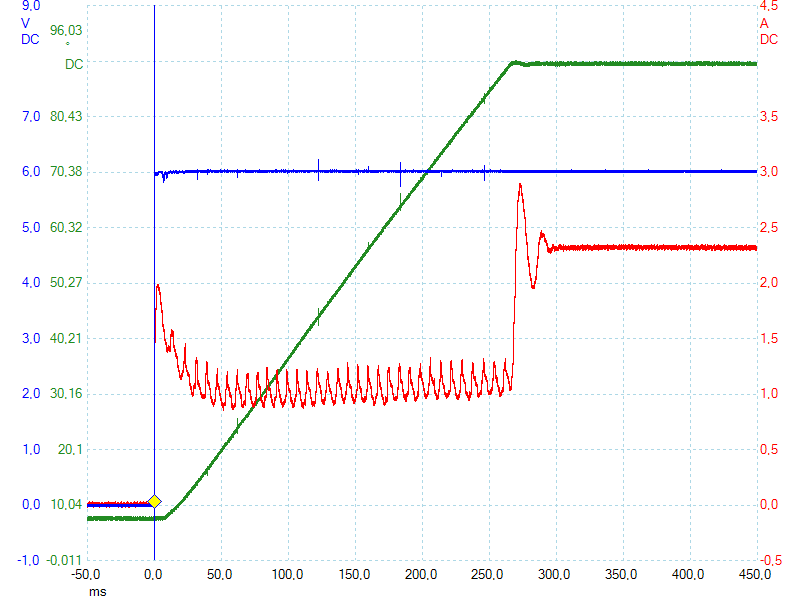
\includegraphics[width=0.50\textwidth,height=3.2cm,keepaspectratio]{oszi_p2_1.png}
\caption{Aufzeichnung des realen Öffnungsvorgangs bei $U = 6\,\text{V}$ (blau: Klemmenspannung $u$, grün: Klappenwinkel $\varphi_{\text{DK}}$, rot: Ankerstrom $I$).}
\label{fig:oszi_6v}
\end{figure}
\vspace{-4mm}
\begin{figure}[H]
\centering
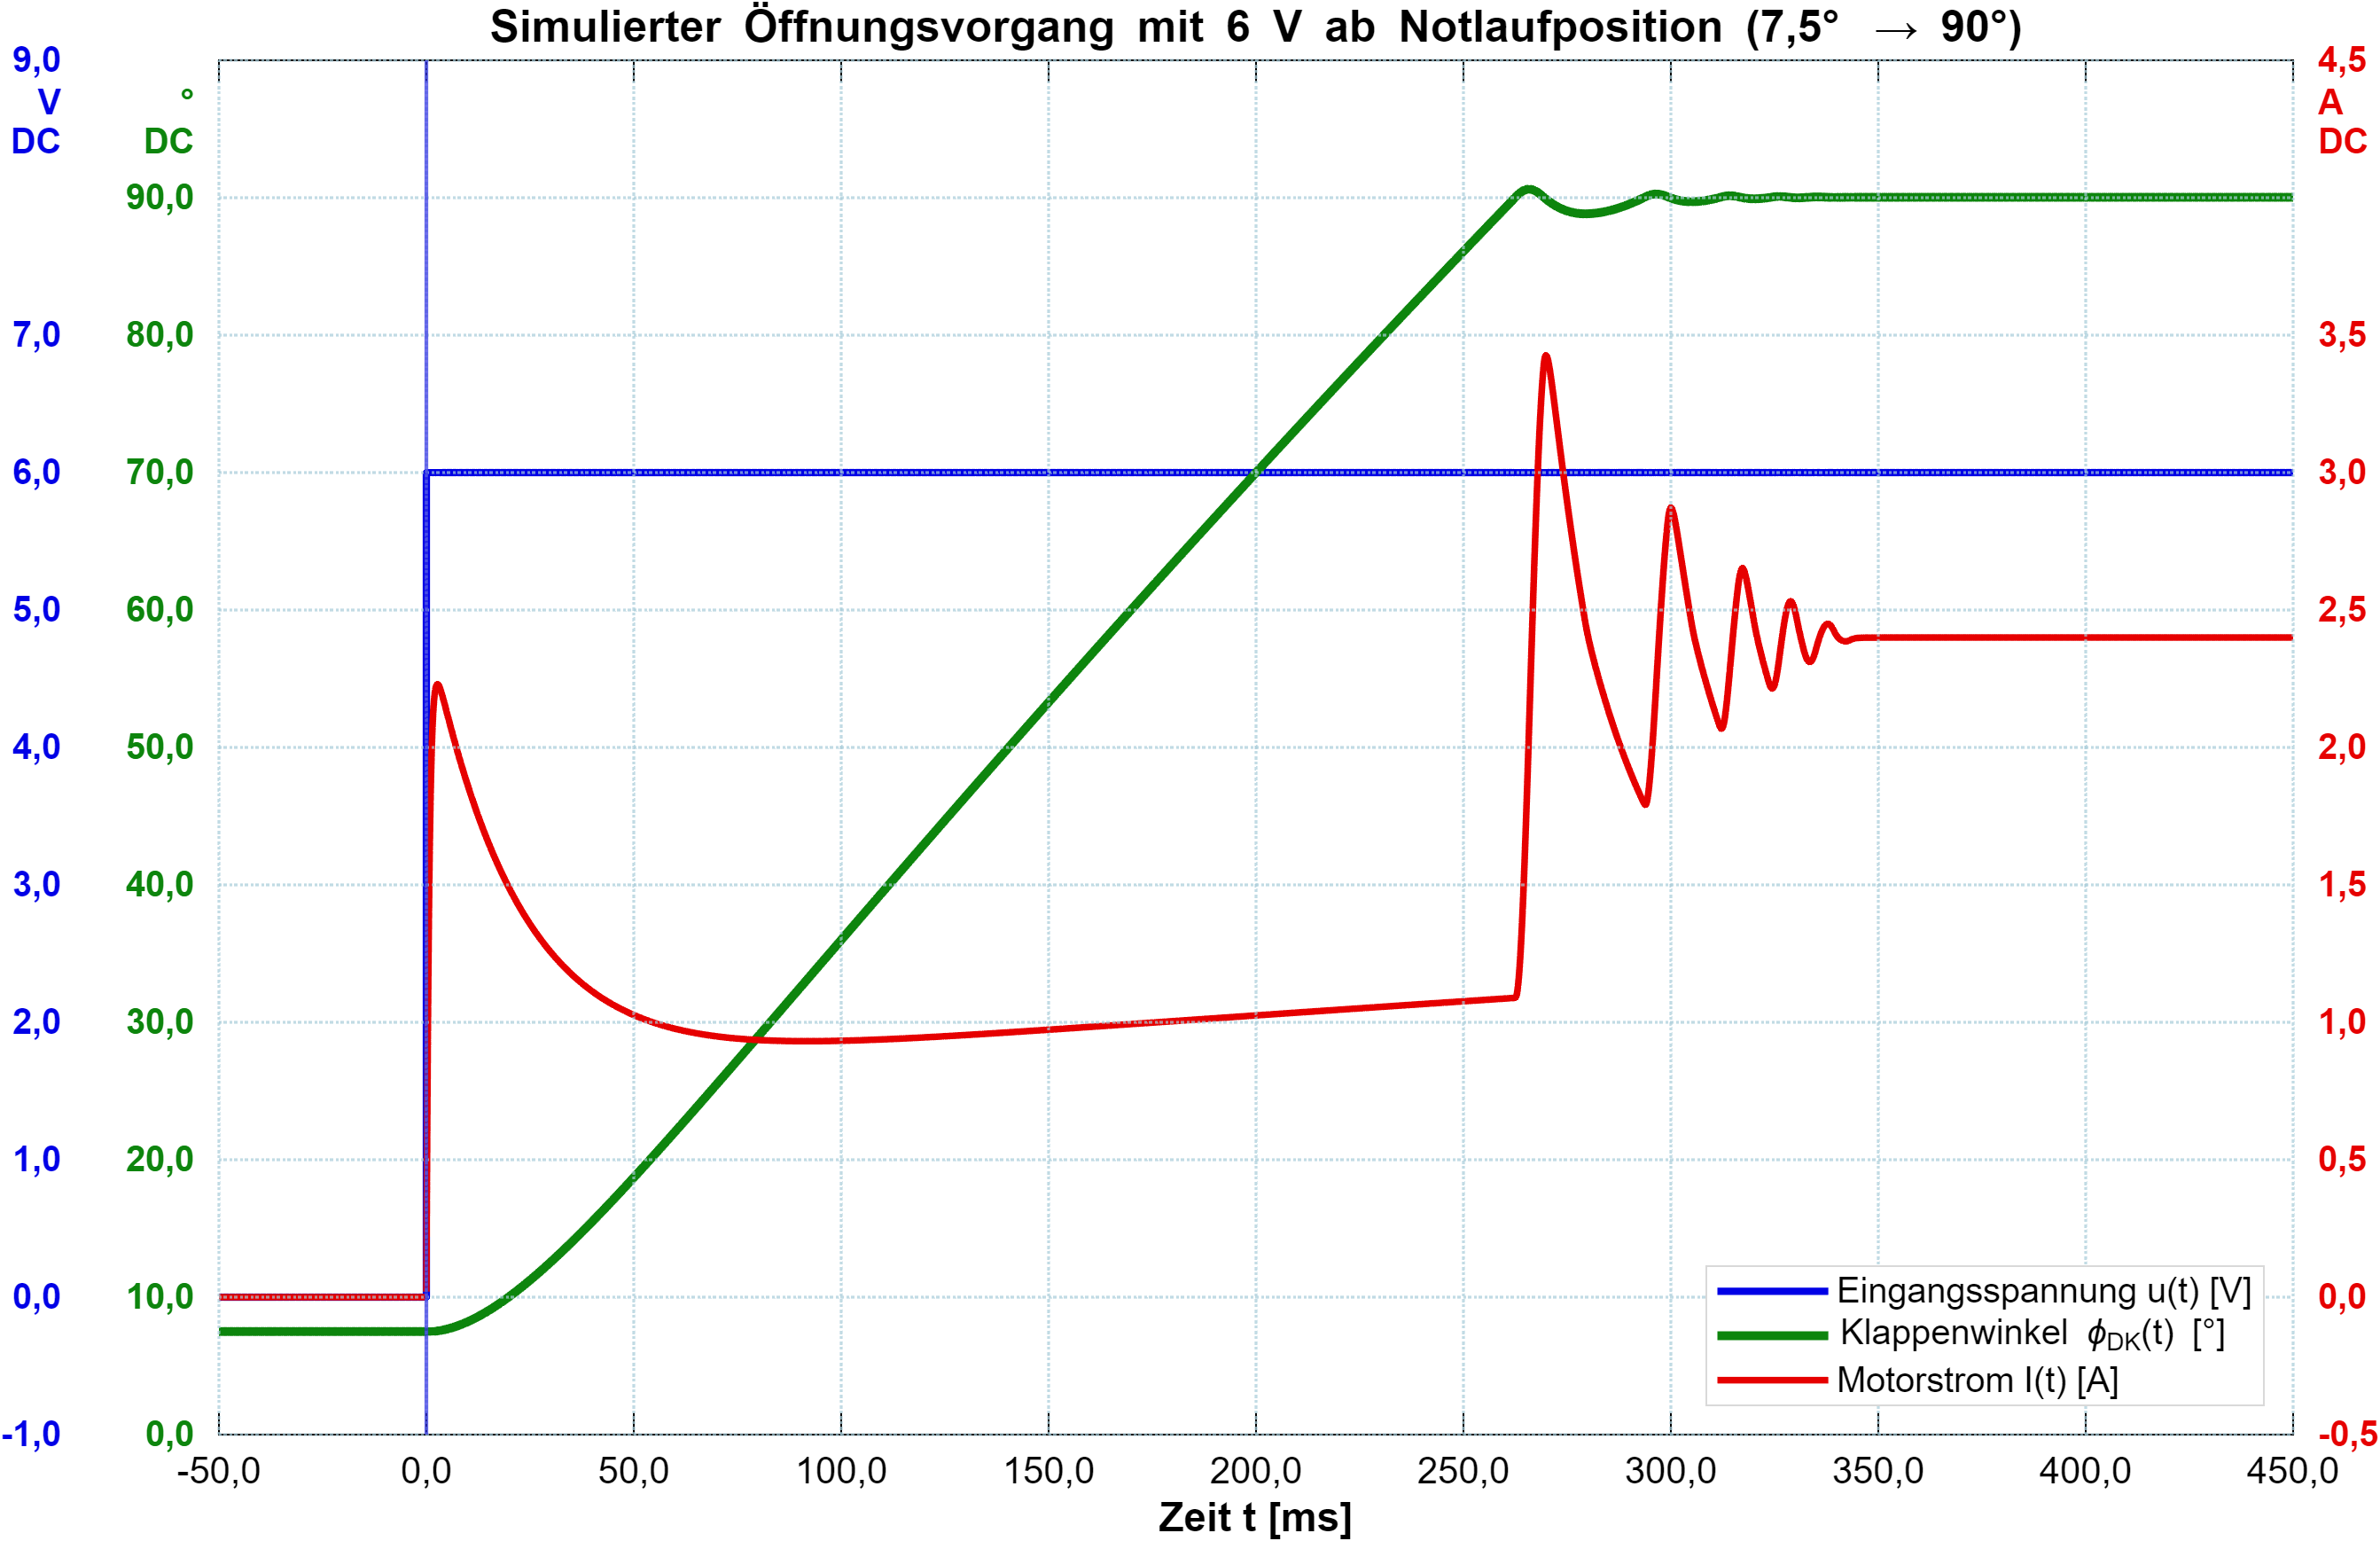
\includegraphics[width=0.54\textwidth,height=3.4cm,keepaspectratio]{plot_drosselklappe_simulation.png}
\caption{Simulierter Öffnungsvorgang des Simulink-Modells bei $U = 6\,\text{V}$ (blau: Eingangsspannung $u(t)$, grün: Klappenwinkel $\varphi_{\text{DK}}(t)$, rot: Motorstrom $I(t)$).}
\label{fig:sim_vergleich}
\end{figure}
\vspace{-3mm}
\begin{itemize}\setlength{\itemsep}{2pt}
    \item \textbf{Zeitverlauf des Klappenwinkels (grüne Kurve):}\\
    Sowohl in der Messung als auch in der Simulation verharrt die Klappe nach dem Spannungssprung bei $t = 0\,\text{ms}$ zunächst kurz in der Notlaufposition bei $7{,}5^\circ$ (ca. $5\dots 8\,\text{ms}$), bis der ansteigende Ankerstrom die Schwelle $I_{\text{start}} = (M_{F,\text{NLP}} + M_R)/k_{\text{Mot}} = 0{,}85\,\text{A}$ zur Überwindung von Federvorspannung und Reibung überschreitet. Danach öffnet die Klappe mit nahezu konstanter Steigung bis zum mechanischen Anschlag bei $90^\circ$. Die simulierte Öffnungszeit von $t_{\text{sim}} \approx 263\,\text{ms}$ stimmt sehr gut mit der realen Messung am Oszilloskop ($t_{\text{real}} \approx 270\,\text{ms}$) überein.
    \item \textbf{Verlauf des Motorstroms (rote Kurve):}\\
    Beim Einschalten ($t = 0\,\text{ms}$) befindet sich der Rotor noch im Stillstand ($u_{\text{EMK}} = 0$), sodass der Strom mit der elektrischen Zeitkonstante $\tau_{\text{el}}$ steil auf eine Einschaltspitze von ca. $2{,}0 \dots 2{,}2\,\text{A}$ ansteigt. Mit zunehmender Drehzahl baut sich die Gegen-EMK ($u_{\text{EMK}} \approx 3{,}5\,\text{V}$) auf und senkt den Strom während der Öffnungsbewegung auf ein nahezu konstantes Plateau von $I_{\text{Fahrt}} \approx 0{,}97\,\text{A}$ (Simulation) bzw. ca. $1{,}0\,\text{A}$ im Mittel der Messung. Beim Erreichen des $90^\circ$-Anschlags wird der Rotor auf $\omega = 0$ abgebremst ($u_{\text{EMK}} = 0$), wodurch der Strom nach einem kurzen Einschwingen am Anschlag auf den stationären Blockierstrom $I_{\text{Block}} = U/R = 2{,}40\,\text{A}$ (real ca. $2{,}32\,\text{A}$) springt.
\end{itemize}

\subsection{Schwächen der Modellierung und Ursachen der Abweichungen}
Die verbleibenden kleinen Abweichungen zwischen Simulation und realer Messung lassen sich auf folgende Modellvereinfachungen zurückführen:
\begin{enumerate}\setlength{\itemsep}{2pt}
    \item \textbf{Erwärmung und Widerstandsänderung:}\\
    Während der Bestromung erwärmt sich die Kupferwicklung des Rotors, wodurch der Widerstand von $R_{\text{kalt}} = 2{,}50\,\Omega$ auf $R_{\text{warm}} = \frac{6{,}0\,\text{V}}{2{,}32\,\text{A}} \approx 2{,}59\,\Omega$ ansteigt und der reale Blockierstrom leicht sinkt.
    \item \textbf{Getriebespiel und Elastizität:}\\
    Beim Anfahren und beim Anschlagen bei $90^\circ$ treten im realen Getriebe Zahnflankenspiel und elastische Verformungen auf (sichtbar am kurzen Nachschwingen des Stroms im Oszilloskop bei $t = 270\dots 290\,\text{ms}$).
    \item \textbf{Magnetische Sättigung und komplexe Reibung:}\\
    Neben konstanter Gleitreibung treten real erhöhte Haftreibung, drehzahlproportionale viskose Reibung, Kommutatorrippel durch die 8 Lamellen sowie magnetische Sättigung bei hohen Strömen auf.
\end{enumerate}



% ##############################################################################
% SEITE 6: TESTFRAGEN & ERKENNTNISGEWINN
% ##############################################################################
\section{Beantwortung der Testfragen und Erkenntnisgewinn}
\subsection{Leitfragen zur Modellbildung und Induktivitätsbestimmung (Kap. 1.4 \& 4)}
\begin{itemize}\setlength{\itemsep}{3pt}
    \item \textbf{Wirkungskette des Gleichstrommotors:}\\
    Aus der Differenz von Eingangsspannung $u$ und Gegen-EMK $u_{\text{EMK}} = k_{\text{EMK}} \cdot \omega$ folgt mit der Übertragungsfunktion des Ankerkreises $F_{\text{el}}(s) = \frac{1/R}{(L/R)s + 1}$ der Motorstrom $I$ (wobei wegen $\tau_{\text{el}} \ll \tau_{\text{mech}}$ oft $L \approx 0 \implies F_{\text{el}}(s) \approx 1/R$ vereinfacht werden kann). Multiplikation mit $k_{\text{Mot}}$ liefert das Antriebsmoment $M_A = k_{\text{Mot}} \cdot I$.
    \item \textbf{Effektives Moment, Drehzahl und Winkelposition:}\\
    Vom Antriebsmoment $M_A$ werden das Reibmoment $M_R(\omega)$ (entgegen der Drehrichtung) und das Federmoment $M_F(\varphi_{\text{DK}})$ (in Richtung Notlaufposition $\varphi_{\text{NLP}} = 7{,}5^\circ$) abgezogen: $M_{\text{eff}} = M_A - M_R - M_F$. Division durch das Massenträgheitsmoment $J$ liefert die Winkelbeschleunigung $\dot{\omega} = M_{\text{eff}}/J$, einfache Integration ($1/s$) die Winkelgeschwindigkeit $\omega$, eine zweite Integration ($1/s$) den Motorwinkel $\varphi_{\text{Mot}}$ und die Skalierung mit $k_{\text{Gr}} \cdot \frac{180^\circ}{\pi}$ den Klappenwinkel $\varphi_{\text{DK}}$ in Grad.
    \item \textbf{Einfluss der EMK:}\\
    Nach dem Induktionsgesetz induziert der rotierende Anker im Permanentmagnetfeld eine zur Drehzahl proportionale Gegenspannung $u_{\text{EMK}} = k_{\text{EMK}} \cdot \omega$, die der Versorgungsspannung entgegenwirkt, den Strom bei steigender Drehzahl begrenzt und wie eine geschwindigkeitsproportionale elektrische Dämpfung wirkt.
    \item \textbf{Zwei Möglichkeiten zur Bestimmung der Induktivität $L$:}\\
    Erstens durch direkte Wechselstrommessung mit einem RLC-Messgerät bei $f = 1\,\text{kHz}$. Zweitens durch Aufzeichnung der Strom-Sprungantwort nach einem Spannungssprung am Oszilloskop bei festgehaltenem Rotor ($\omega = 0$), Ablesen der elektrischen Zeitkonstante $\tau_{\text{el}}$ und Berechnung über $L = R \cdot \tau_{\text{el}}$.
\end{itemize}

\subsection{Simulink-Testsystem mit \texorpdfstring{$F(s) = \frac{5}{2s^2 + 8}$}{F(s) = 5 / (2s\^2 + 8)} bei Sprung \texorpdfstring{($0 \to 5$)}{(0 -> 5)}}
Die Übertragungsfunktion $F(s) = \frac{5}{2s^2 + 8} = \frac{5/8}{\frac{1}{4}s^2 + 1}$ beschreibt ein ungedämpftes $\text{PT}_2$-Schwingungsglied ($D = 0$, rein imaginäre Pole bei $s_{P1,2} = \pm j\,2\,\text{s}^{-1}$) mit dem statischen Übertragungsfaktor $K = \frac{5}{8} = 0{,}625$ und der Eigenkreisfrequenz $\omega_0 = \sqrt{8/2} = 2\,\text{rad/s}$ (Periodendauer $T_0 = \frac{2\pi}{\omega_0} = \pi\,\text{s} \approx 3{,}142\,\text{s}$). Bei einem Eingangssprung der Höhe $\Delta u = 5$ schwingt das Ausgangssignal $y(t) = 3{,}125 \cdot \bigl(1 - \cos(2\,(t - t_0))\bigr)$ ungedämpft zwischen $y_{\text{min}} = 0$ und $y_{\text{max}} = 2 \cdot K \cdot \Delta u = 6{,}25$ um den stationären Mittelwert $y_m = K \cdot \Delta u = 3{,}125$ (Abbildung~\ref{fig:testfrage_sim}).

\begin{figure}[H]
\centering
\begin{minipage}[c]{0.36\textwidth}
    \centering
    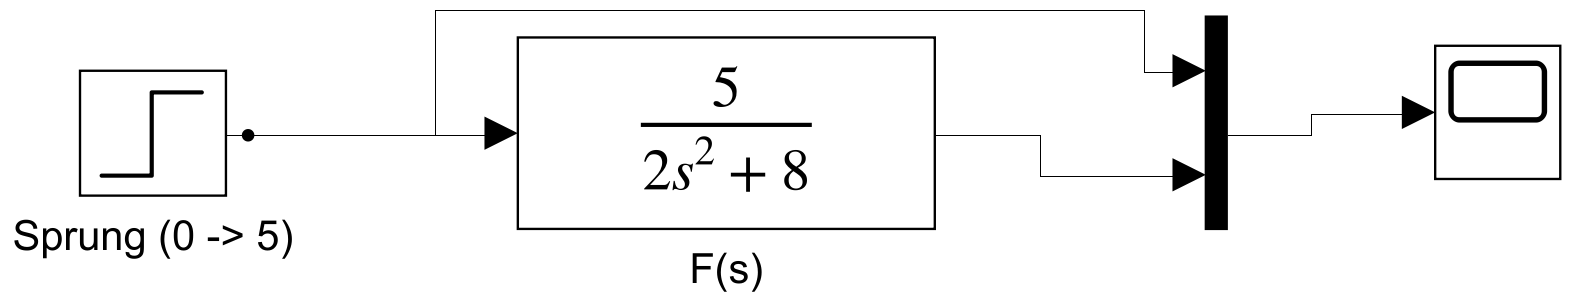
\includegraphics[width=\textwidth,height=3.2cm,keepaspectratio]{simulink_testfrage.png}
\end{minipage}\hfill
\begin{minipage}[c]{0.62\textwidth}
    \centering
    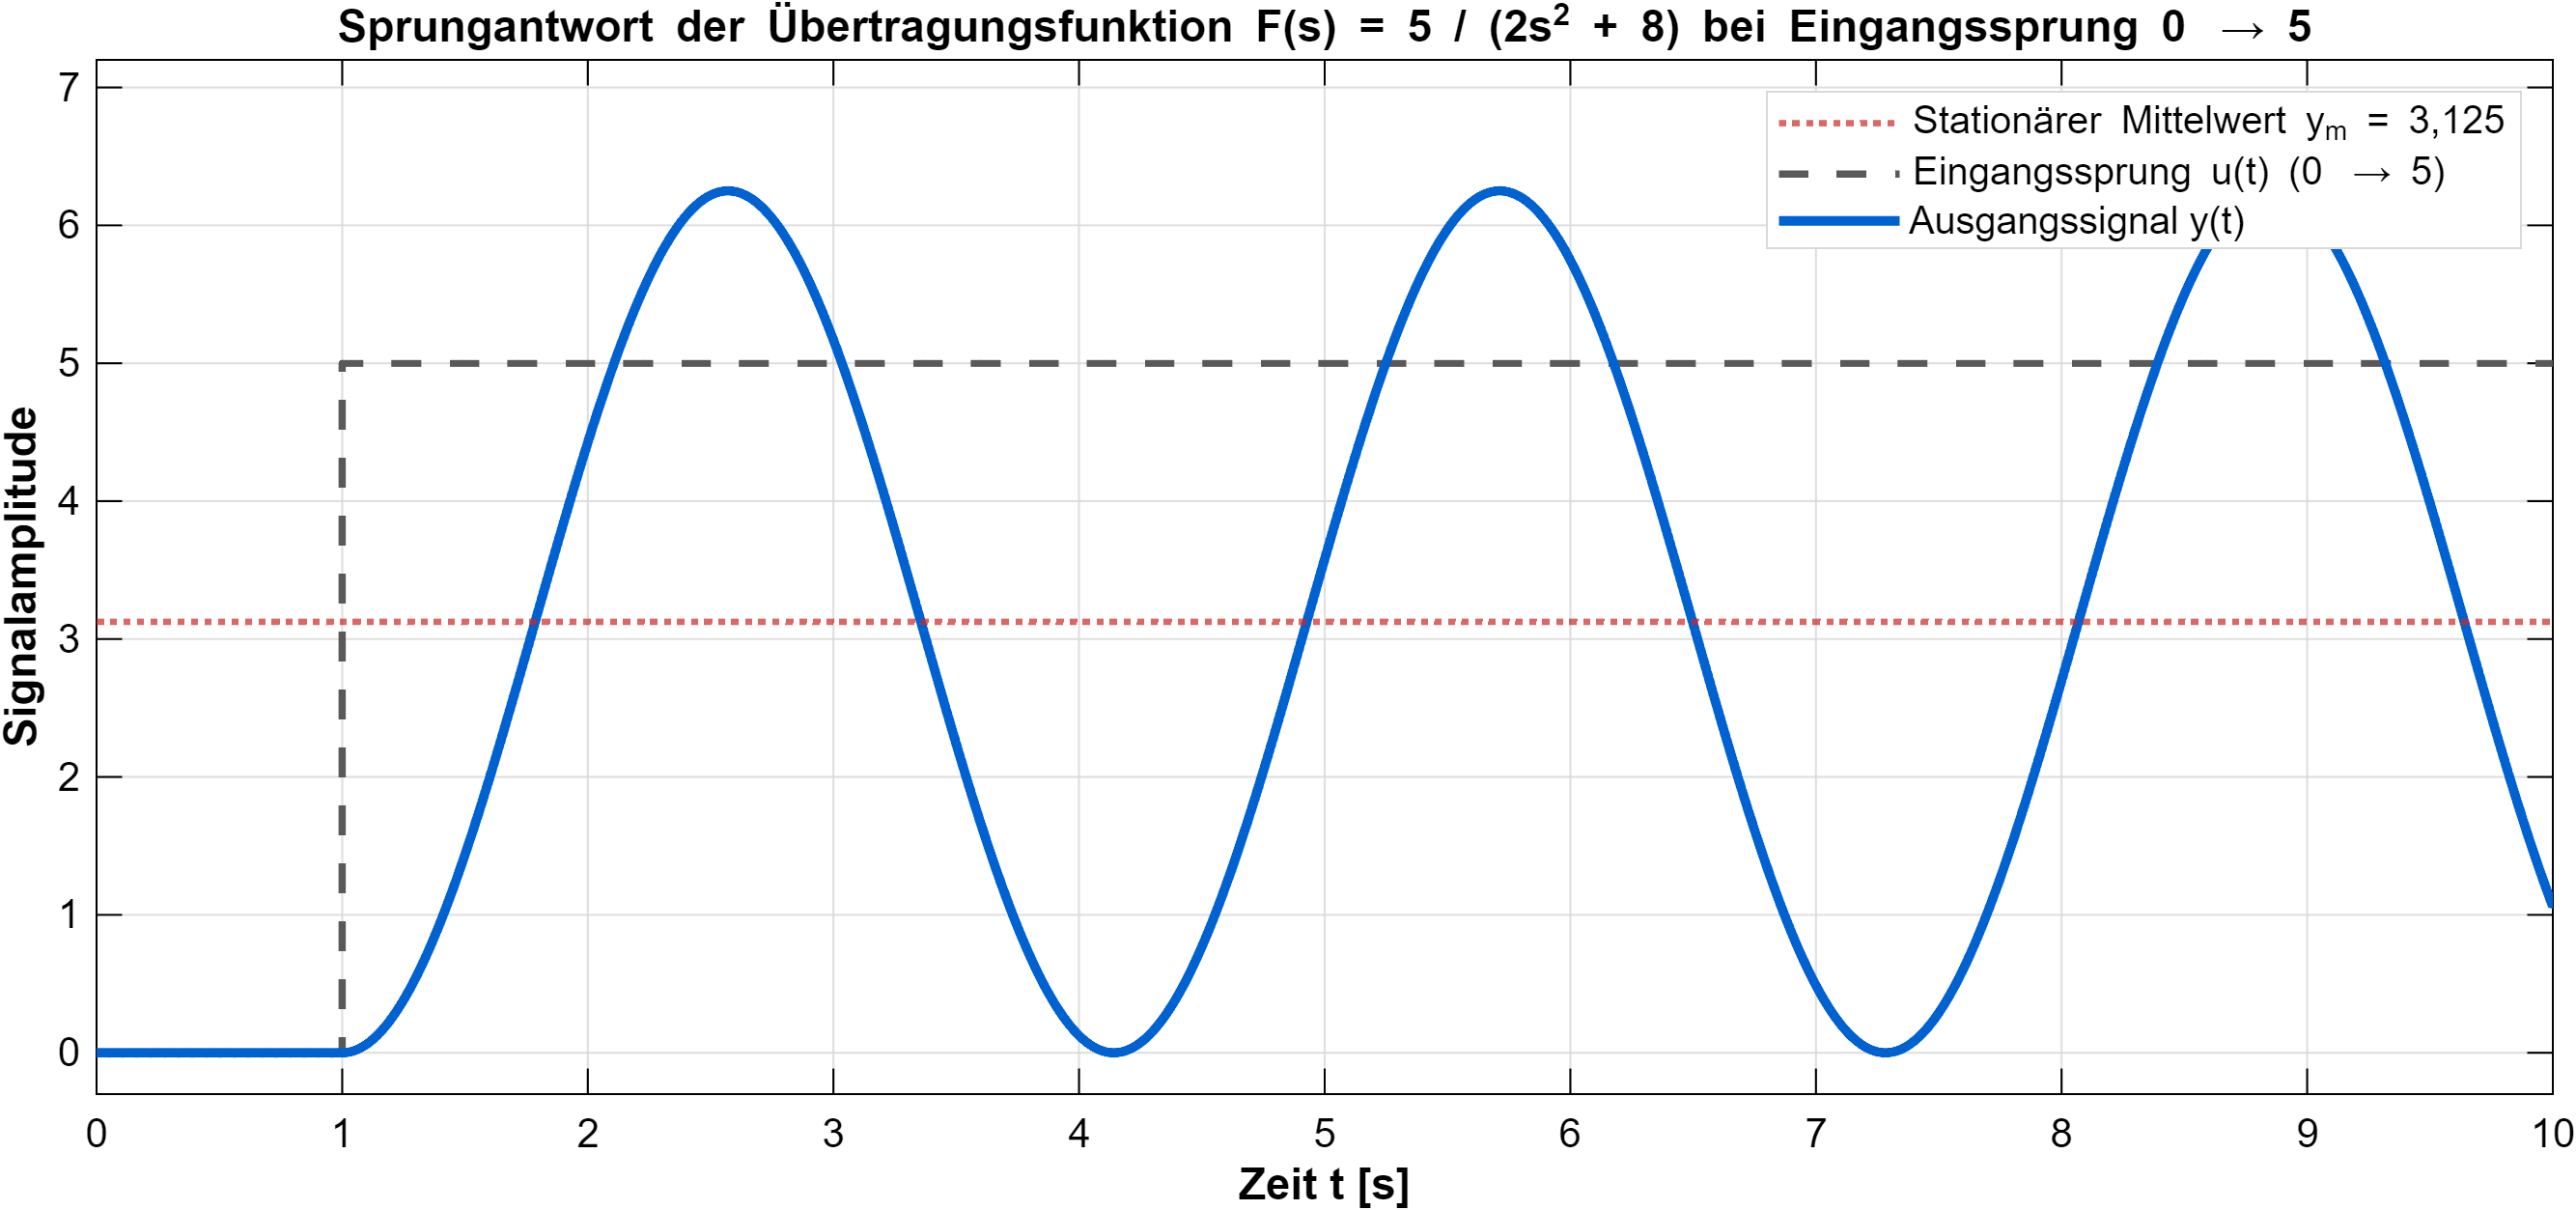
\includegraphics[width=\textwidth,height=3.5cm,keepaspectratio]{plot_testfrage_simulation.png}
\end{minipage}
\caption{Simulink-Modell (links) und simulierte Sprungantwort (rechts) von $F(s) = \frac{5}{2s^2 + 8}$ bei einem Eingangssprung $0 \to 5$.}
\label{fig:testfrage_sim}
\end{figure}

\subsection{Fazit}
Bereits ein strukturell übersichtliches physikalisches Modell bildet das reale dynamische Öffnungsverhalten der Drosselklappe sehr präzise ab, sofern die dominanten Nichtlinearitäten (Momentensprung der Notlauffeder bei $7{,}5^\circ$ und vorzeichenrichtige Festkörperreibung) sowie das quadratische Übersetzungsverhältnis bei den Trägheiten ($J \approx J_{\text{Rotor}}$) berücksichtigt werden. Zudem zeigt der Versuch, dass einfache analytische Plausibilitätsprüfungen ($k_{\text{Mot}} \approx k_{\text{EMK}}$ im SI-System, $M_F > M_R$ für Fail-Safe und $M_{M,\text{max}} > M_F + M_R$) unverzichtbar sind, um Vorzeichen- oder Skalierungsfehler (wie einen vergessenen Getriebefaktor $k_{\text{Gr}}$) schon vor dem ersten Simulationslauf zuverlässig zu erkennen.

\label{doc:lastpage}
\end{document}
